\documentclass{book}
\usepackage[utf8]{inputenc}
\usepackage{graphicx}
\title{Neural Networks for Machine Learning}
\author{Huynh Xuan Phung - Coursera}
\date{ }
\usepackage{color}   %May be necessary if you want to color links
\usepackage{hyperref}
\hypersetup{
    colorlinks=true, %set true if you want colored links
    linktoc=all,     %set to all if you want both sections and subsections linked
    linkcolor=blue,  %choose some color if you want links to stand out
} 
\begin{document}
 
\maketitle
 
\tableofcontents

\chapter{Introduction}

Why is Machine Learning?

It is hard to write the program to compute and recognize

\chapter{Perceptrons}

\section{Type of network}

-- Feed-forward neural network: more hidden layers: deep. They compute a series

-- Recurrent network: have directed cycles in their connection graph; complicated dynamics; biological

----- remember information

-- Symmetrically connected networks: John Hopfield
\section{Perceptron}

The first generation of neural networks

The standard paradigm of statistical pattern recognition:

--- Convert the row input into a vector of features activation

--- Learn how to weight each of the feature activation to get the single scalar quantity

--- set the threshold

Binary thresh neurons (decision units)

Learning procedure:

--- add an extra component with value 1 to each input: bias

--- Pick training case using any policy that ensure that every training case will keep getting picked

------ If the output unit is correct, leave its weight alone

------ If the output unit is incorrectly outputs a zero, add the input vector to the weight vector

------ If the output unit is incorrectly outputs a one, subtract the input vector from the weight vector (w = w - input)

\section{Geometrical view of perceptron}

\subsection{Weight-space}
has one dimension per weight

\begin{figure}[h]
\centering
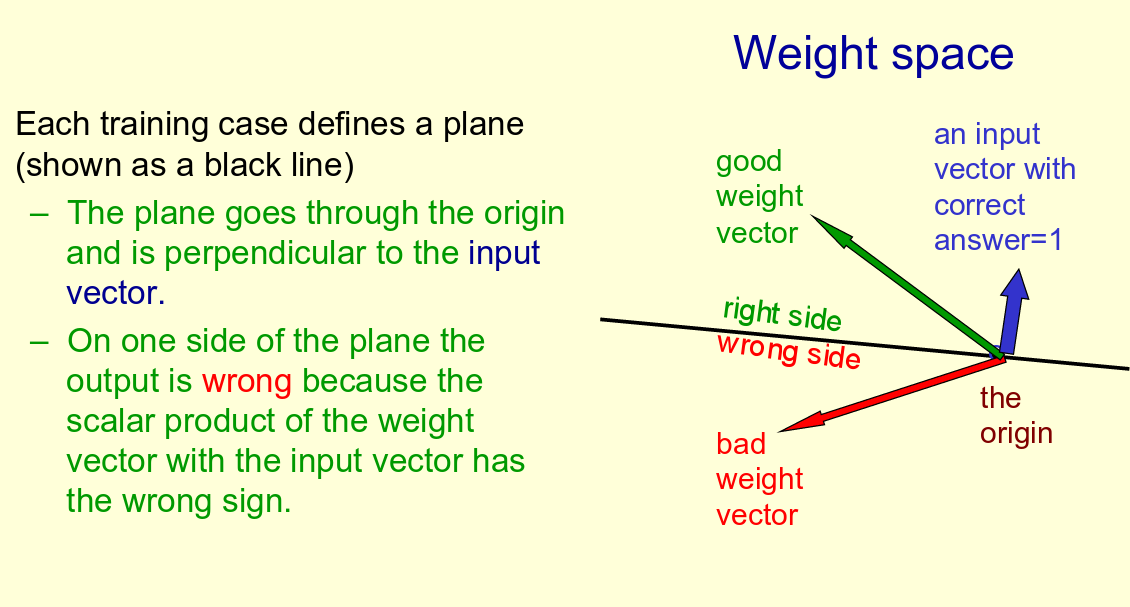
\includegraphics[width=0.7\linewidth]{./figures/weightplane}
\caption{The weight space view}
\label{fig:weightplane}
\end{figure}
 
 The problem is convex if average of any 2 solution also a solution


 

\end{document}